The following section consists of three parts. The first one is a brief introduction to C\&C models. The tools used for this study follow up second. Lastly, the used case study method is presented.

\subsection{C \& C models}

In the following a short introduction in Connector and Component (C\&C) model based software development is given. C\&C modeling divides a task into Components and Connectors.

A \emph{Component} represents a computation. It has predefined inputs and outputs, where the output data is obtained by some kind of mathematical transformation of the input data. A \emph{Connector} represents interaction mechanisms by connecting outputs with inputs. By making this division, the paradigm ensures modularity and therefore re-usability.
It can be used for modeling software with high demands for testing and verification such as software for self-driving vehicles \cite{WencksternCCViP}\cite{WencksternSimFrame}.
Another benefit is that a graphical representation is always possible and more efficiently obtainable compared to other text based development, especially non model driven development. The structure of C\&C models also benefits code generation techniques in order to transform models into source code for various target systems.
Well established examples of C\&C modeling and development are SysML\cite{sysml}, AADL\cite{aadl}, Simulink\cite{simulink} and Labview\cite{labview}. The latter two are used in the automotive domain to model behaviour of Electronic Control Units (ECUs) and test their functionality.

\subsection{MontiCore and EmbeddedMontiArc}

MontiCore \cite{HR17}, MontiCAR \cite{KRRW17} and EmbeddedMontiArc \cite{HKK+18} are tools developed by the Chair of Software Engineering of RWTH Aachen University\cite{serwth}.
\emph{MontiCore} is a language workbench intended for agile and model-driven software development. Its primary objective is to enable efficient development of Domain Specific Languages (DSLs) which enhance the development process for Domain Experts. 
\emph{MontiCAR} is a composition of such DSLs, used as an language set for Cyber-Physical Systems \cite{seminarArmin}. Figure \ref{fig:MontiCAR} shows the DSLs which are part of MontiCar and their respective connections.
\begin{figure}
	\centering
	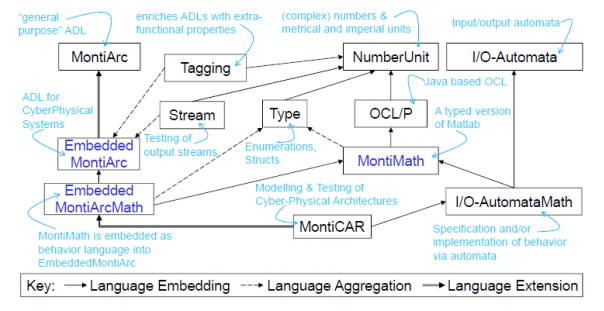
\includegraphics[scale=0.55]{pictures/MontiCarOverview.PNG}
	\caption{Composition of MontiCAR language family\cite{seminarArmin}}
	\label{fig:MontiCAR}
\end{figure}
The components directly used in this studies implementation are EmbeddedMontiArc, EmbeddedMontiArcMath and Stream.
\emph{EmbeddedMontiArc} represents the core language of MontiCar. It implements a C\&C DSL which can be used to write C\&C models, verify, test and deploy them to another architecture. Due to its modularity different simulators and Stream tests can be integrated. See the chapter modeling for more information. Figure \ref{fig:EMontiArc} depicts a usage of the EmbeddedMontiArc DSL.

\begin{figure}[!h]
	\centering
	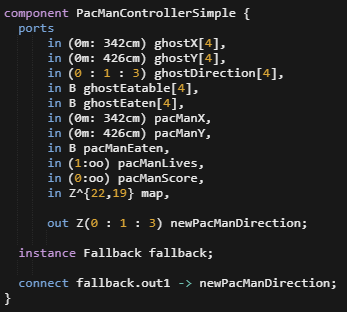
\includegraphics[scale=0.70]{pictures/EMA.PNG}
	\caption{Example Component with Connectors}
	\label{fig:EMontiArc}
\end{figure}

\emph{EmbeddedMontiArcMath} is a DSL for implementing mathematical expressions, thus used for transforming the input values of a Component into its output values. It is also able to declare other variables than the defined inputs and logical structures like if-statements and loops. Example usage of EmbeddedMontiArcMath is shown in figure \ref{fig:EMontiArcMath}.

\begin{figure}[!h]
	\centering
	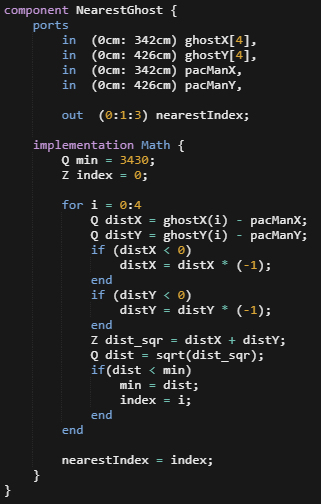
\includegraphics[scale=0.7]{pictures/EMAMath.PNG}
	\caption{Example EmbeddedMontiArcMath implementation}
	\label{fig:EMontiArcMath}
\end{figure}

The \emph{Stream} DSL allows to implement test cases by defining the expected output values for a given input. Multiple values can be tested in one Stream test, as shown in figure \ref{fig:EMAStream} which shows an example stream test for a sum function.

\begin{figure}[!h]
	\centering
	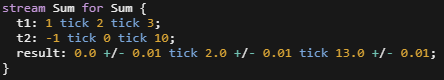
\includegraphics[scale=0.7]{pictures/EMAStream.PNG}
	\caption{Example Stream implementation]}
	\label{fig:EMAStream}
\end{figure}



\subsection{Performing a Case Study in Software Engineering}
This study roughly follows the guidelines stated by Runeson and Hoest \cite{CaseStudyGuidelines} by presenting the objective, the specific case, method and acquiring both quantitative and qualitative data. Quantitative data is acquired by asking a set of predefined questioned and answering them on a scale from 1 to 10. The qualitative data is obtained via requiring subjects to formalize how they gave the quantitative rating.
The quantitative data is analyzed by calculating the mean of each question, and the quantitative by summarizing the subject's writings.
